\section*{Overview}

Link-cut trees maintain a dynamic forest under rerooting, linking, cutting, and path queries. They are one of the few
structures in contest programming that really feel layered: the public API talks about trees, but the implementation is
powered by splay trees over preferred paths.

This is an advanced note because both the idea and the debugging burden are real. Still, once the structure clicks, it
becomes one of the cleanest ways to handle dynamic-tree path queries in \(O(\log n)\) amortized time.

\section*{When to Use It}

Use a link-cut tree when:

\begin{itemize}
  \item the forest changes over time,
  \item queries are about paths rather than static subtrees,
  \item you need operations like \texttt{link}, \texttt{cut}, \texttt{make\_root}, or path aggregate queries,
  \item heavy-light decomposition is not enough because the represented tree itself is dynamic.
\end{itemize}

If the tree is static, heavy-light decomposition is usually much easier to trust and implement.

\section*{Core Idea}

The represented forest is decomposed into \emph{preferred paths}. Each preferred path is stored as one auxiliary splay
tree.

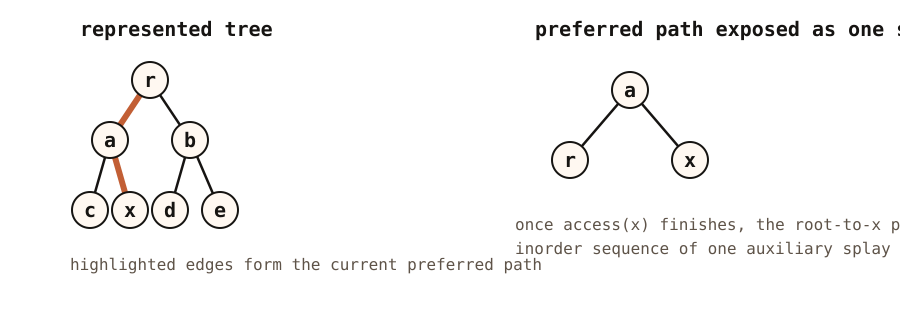
\includegraphics[width=\textwidth]{figures/preferred-paths.svg}

The central operation is \texttt{access(x)}. It repeatedly walks toward the represented root and rewires preferred
paths so that the final preferred path from the represented root to \(x\) becomes explicit.

After that exposure, path operations become splay-tree operations on one auxiliary tree.

\section*{Key Insight}

The phrase that made link-cut trees readable to me is:
\textbf{a link-cut tree is a splay tree data structure for root-to-node exposure}.

Everything revolves around exposing a path:

\begin{itemize}
  \item \texttt{access(x)} makes the root-to-\(x\) path preferred,
  \item \texttt{make\_root(x)} is basically expose + reverse,
  \item path queries between \(u\) and \(v\) become ``reroot \(u\), then expose \(v\)''.
\end{itemize}

So the structure is not maintaining all simple paths directly. It keeps changing which paths are represented
explicitly, depending on what was accessed last.

\section*{Operations / Main Technique}

The standard operations are:

\begin{itemize}
  \item \textbf{access(x)}: expose the represented root-to-\(x\) path,
  \item \textbf{make\_root(x)}: reroot the represented tree at \(x\),
  \item \textbf{find\_root(x)}: find the represented root of \(x\)'s tree,
  \item \textbf{link(x, y)}: connect two different trees,
  \item \textbf{cut(x, y)}: remove one represented edge,
  \item \textbf{connected(x, y)}: test whether two vertices lie in the same tree,
  \item \textbf{path\_query(x, y)}: query an aggregate on the path.
\end{itemize}

\paragraph{Worked path query.}
To query the path from \(u\) to \(v\):

\begin{enumerate}
  \item call \(\texttt{make\_root(u)}\),
  \item call \(\texttt{access(v)}\),
  \item splay \(v\),
  \item now the auxiliary splay rooted at \(v\) represents exactly the path from \(u\) to \(v\).
\end{enumerate}

So if each splay node stores a path aggregate, the answer is sitting at that auxiliary root.

\section*{Correctness Intuition}

The auxiliary splay trees are not arbitrary partitions of the represented tree. Each auxiliary tree corresponds to one
preferred path, and \texttt{access} is the operation that changes which child edge is preferred at each step upward.

After \(\texttt{make\_root(u)}\), vertex \(u\) becomes the represented root. Then \(\texttt{access(v)}\) exposes the
entire path from \(u\) to \(v\) as one preferred path. Since the path is now explicit inside a single auxiliary splay
tree, any maintained path aggregate is correct after the usual splay push/pull routines.

\section*{Complexity Analysis}

\begin{itemize}
  \item \texttt{access}, \texttt{make\_root}, \texttt{link}, \texttt{cut}, path queries: \(O(\log n)\) amortized,
  \item memory: \(O(n)\).
\end{itemize}

The amortization comes from the splay-tree layer. Link-cut trees inherit both the power and the caveats of splaying.

\section*{Implementation}

The reference code keeps a deliberately limited but useful version:

\begin{itemize}
  \item vertex values,
  \item path sums,
  \item link, cut, connected, reroot, and point update.
\end{itemize}

It does not attempt subtree aggregates or heavy lazy propagation. Those are possible, but they add a second layer of
difficulty and deserve their own careful pass.

\section*{Common Pitfalls}

\begin{itemize}
  \item Building on top of a splay implementation that is not fully reliable.
  \item Forgetting to push the reversal flag before rotations or before walking down the tree.
  \item Confusing the represented-tree parent with the auxiliary-tree parent.
  \item Forgetting that \texttt{access} changes preferred paths globally, not just locally at one node.
  \item Trying to answer subtree queries with a path-only implementation.
\end{itemize}

\section*{Variants / Extensions}

\begin{itemize}
  \item path xor, min, max, or other associative aggregates,
  \item subtree information by tracking virtual subtrees,
  \item lazy path updates,
  \item dynamic MST or replacement-edge style applications.
\end{itemize}

The structure stays conceptually the same: expose paths with link-cut operations, and let the auxiliary splay nodes
store the right summary.

\section*{Practice Problems}

\begin{itemize}
  \item Dynamic forest connectivity with link and cut.
  \item Dynamic path sum or xor queries.
  \item Problems where edges appear and disappear over time and the maintained answer depends on tree paths.
\end{itemize}

\section*{References}

\begin{itemize}
  \item \href{https://usaco.guide/adv/link-cut-tree?lang=cpp}{USACO Guide: Link-Cut Tree}.
  \item \href{https://www.researchgate.net/publication/221590599_A_Data_Structure_for_Dynamic_Trees}{Sleator and Tarjan: A Data Structure for Dynamic Trees}.
  \item \href{https://zhtluo.com/cp/splay-tree-one-tree-to-rule-them-all.html}{Zhtluo: Splay Tree - One Tree to Rule Them All}.
  \item \href{https://codeforces.com/catalog}{Codeforces Catalog}.
\end{itemize}
